
%(BEGIN_QUESTION)
% Copyright 2006, Tony R. Kuphaldt, released under the Creative Commons Attribution License (v 1.0)
% This means you may do almost anything with this work of mine, so long as you give me proper credit

En enkel type elektronisk trykktransmitter kan bygges med et bourdon-rør og en \textit{Linear Variable Differential Transformer}, eller \textit{LVDT}:

$$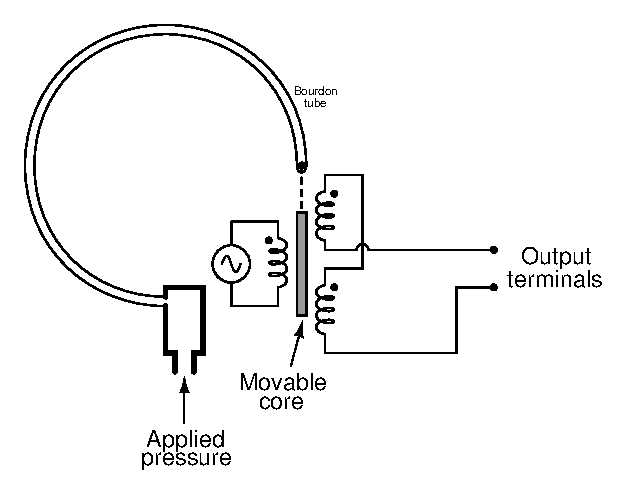
\includegraphics[width=15.5cm]{i00183x01.eps}$$

Forklar hvordan dette instrumentet virker, hvilken type elektrisk utgangssignal det genererer (f.eks. strøm, spenning, motstand osv.), og hvilken polaritet (om noen) utgangssignalet har.

\underbar{file i00183}
%(END_QUESTION)





%(BEGIN_ANSWER)

Legg nøye merke til hvordan de to sekundærviklingene er koblet i seriemotfase (markert med faseprikker).  Denne detaljen er avgjørende for å forstå hvordan LVDT-en virker.

\vskip 10pt

Utgangen er en AC-spenning med amplitude proporsjonal med kjernens posisjon, som igjen er proporsjonal med pålagt trykk.  Fasen til utgangsspenningen vil snu i forhold til eksitasjonsspenningen når bourdon-røret trekker kjernen opp:

$$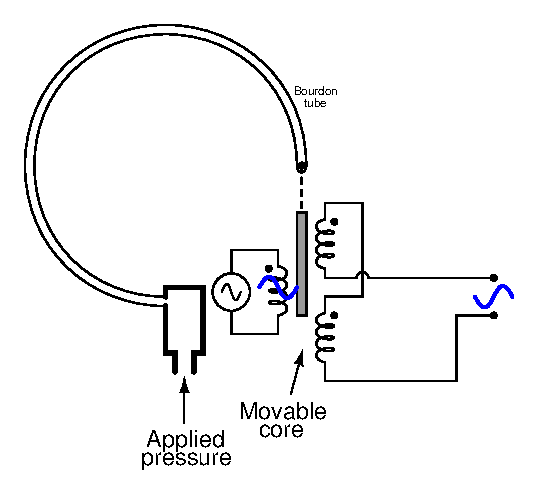
\includegraphics[width=15.5cm]{i00183x02.eps}$$

LVDT-er har flere fordeler sammenlignet med potensiometre:

\begin{itemize}
\item{} Ingen friksjon
\item{} Ingen slitasje
\item{} Ingen tendens til gnistdannelse under normal drift
\end{itemize}

Den største ulempen er at de krever AC-eksitasjonsspenning.  Frekvensen til eksitasjonen er også viktig: den må være mye høyere enn høyeste frekvens på trykkendringer du vil måle (i henhold til Nyquist-teoremet).

%(END_ANSWER)





%(BEGIN_NOTES)

%INDEX% Measurement, pressure: LVDT as bourdon tube sensor

%(END_NOTES)

